\documentclass[../main.tex]{subfiles}
\graphicspath{{\subfix{..}}}
\begin{document}
\chapter{Graph representation of JUNO for IBD reconstruction}
\label{sec:jgnn}
\epigraph{``The Answer to the Great Question of Life, the Universe and Everything is Forty-two''}{Douglas Adams, The Hitchhiker’s Guide to the Galaxy}

\minitoc
%\begin{itemize}
%  \item Introduce the concpet of reconstruction using Small + Large
%  \item Re state the context
%\end{itemize}


In Section \ref{sec:juno:ml}, we showed that all ML methods developed before this thesis to reconstruct IBDs have similar results, and that their performance is very similar to that of the classical, likelihood-based algorithm.
We think these similarities can reasonably be explained by this: the input data used by all these methods to compute $E$ or $\vec{X}$  is the same full list of PMT integrated signals $ \{ (Q_i,t_i) ; ~ i \in  1, ..., N_{PMTs} \}$, and by the high level of sophistication of the detector's description in the likelihood. It's probable that the likelihood method looses very little information.

May be some was, but that the ML algorithms were not desgined well enough to recover it. It's also reasonable to think that ML algorithms will make a difference when, instead of the list of $(Q_i, t_i)$, a rawer information will be used in input, like the full waveform.
To actually be able to learn from such a complex and high dimensional input, well designed architectures (that would guide the learning toward the solution) are necessary. In any case, it seemed welcome to us to propose an additional algorithm, with an original architecture.

For the fist stage of its development, the purpose of this part of my thesis, we considered it was enough to also take the $(Q_i, t_i)$ list as the input.
While achieving equivalent performance with simpler input might suggest that the architecture is not immediately advantageous, it remains crucial to explore the performance with more complex, rawer inputs such as full waveforms. This is where the true potential of the architecture could emerge, as it could better capture the intricacies that simpler inputs fail to represent. If performance does not improve with these richer inputs, it would then be appropriate to question the relevance of this approach.

The algorithm we propose is a GNN. It also has the advantage of addressing sphericity issues described in Chapter \ref{sec:jcnn}.
From this graph representation, we can construct a neural network that will process the data while keeping some interesting properties. For example the rotational invariance, i.e. the energy and
radius of the event do change by rotation our referential. For more details see Section \ref{sec:ml:gnn}. Graph representation also has the advantage to be able to encode global and higher order informations.

%An approach was already proposed in JUNO by Qian et al. \cite{qian_vertex_2021} where each nodes of the graph are like pixels, they represent geometric region of the detector and are connected with their neighbours. The LPMT informations are then aggregated on those nodes. The network then process the data using the equivalent of convolution but on graph \cite{defferrard_convolutional_2017}.
%
%In this work we want to take a step further in the graph representation by including the SPMT and representing PMTs directly as nodes.

\section{Data representation}
\label{sec:jgnn:data}
%\begin{itemize}
%  \item First though
%    \begin{itemize}
%      \item All pmt are nodes
%      \item How to connect ? Fully connected ?
%      \item Fully connected not possible with our computng capacities: 40k * 40k -> $1.6\cdot10^8$ link -> around a Gb of adjacency matrix times edges features
%      \item Connected to neighbours -> Already done for graph convolution, cit yury paper
%    \end{itemize}
%  \item Second though
%    \begin{itemize}
%      \item Be smarter
%      \item All PMTs as nodes -> Fired
%      \item Have intermediate layer of node representing geometric section -> Mesh
%      \item Fired connected to mesh
%      \item Mesh fully connected
%      \item Aggregation while keeping raw informations
%      \item Add a "global node"
%    \end{itemize}
%  \item Present healpix for the segementation
%  \item Features for node/edges
%    \begin{itemize}
%      \item Classic infos: Q,t,X,Y,Z (add plots to show features)
%      \item Add high order informations
%      \item Harmonic analysis (present here ? Or in annex ?)
%      \item Other high order $\mathcal{A}$ and $\mathcal{B}$
%    \end{itemize}
%  \item Difficulty: nodes do not live in the same space (not same infos on fired, mesh, and io)
%  \item Need a custom message passing options
%\end{itemize}


In Section \ref{sec:juno:ml}, we mentioned a GNN developed before the beginning of this thesis to reconstruct IBD energies in JUNO \cite{qian_vertex_2021}. In their approach:
nodes of the graph correspond to 3072 pixels representing geometric regions of the detector and the information of the $\sim6$ LPMTs found in a pixel are then aggregated on those nodes.This aggregation serves to simplify the data input, though at the potential cost of losing finer-grained details.
The network then process the data using the equivalent of convolution but on graph \cite{defferrard_convolutional_2017}. In the first layer, each node is connected only with its direct neighbours.

To determine the energy released by an IBD in the LS, it is helpful to determine the position of the main energy deposit. Therefore, relative Q and t's of PMTs all around the sphere is a useful information. If in the first layer only neighbour nodes are linked, several layers are necessary to access this detector-wide information. In an ideal world, we would develop a Graph NN where each PMT is a node
(even if it has not been hit in the event under consideration, since this is in itself an information) and where each node is connected to all the other ones. This makes the detector-wide information avalaible as early as the first layer. This architecture
might help the network to better learn. Such an architecture can also be motivated this way: one of the strength of GNN's is their capacity to encompass the characteristics of a detector.
A node can be the representation of a detector element, and the edge can represent its relationship with other elements. In the case of JUNO, any measurement is collective : an interaction is seen by all the PMTs, with no a priori hierarchy in the role of each.
A fully connected GNN is particularly advantageous in JUNO's case, as the lack of a priori hierarchy among the PMTs makes it important to ensure that information is shared globally from the outset. This architecture allows the network to access detector-wide information as early as the first layer, potentially improving learning efficiency. However, this comes at a significant computational cost, which necessitates careful balancing between memory usage and model performance

Another advantage of a GNN is also that it is well adapted to inhomogenous detectors.
We therefore tried to build GNNs including both LPMTs ans SPMTs.

With 17612 LPMTs and 25600 SPMTs, the ideal fully connected Graph mentioned above is impossible: even excluding self relation and considering the relation to be undirected (the edge from a node A to a node B being the same from
as the one from B to A) the amount of necessary edges would be $n(n-1)/2$ with $n = 43212$
nodes. This amounts to 933'616'866 edges. If we encode an information with double precision (64 bits) in what we call an adjacency matrix, illustrated in Figure \ref{fig:ml:gnn:graph}, each information we want to encode in the relation would consume 4 GB of data. When adding the overhead due to gradient computation during training, this would put us over the memory capacity of a single V100 gpu card (20 GB of memory).
We could use parallel training to distribute the training over multiple GPU but we considered that the technical challenge to deploy this solution was too high.

%In an ideal world we would like to have every PMTs represented as node in the graph, each PMT being hit is an informations but the fact that PMTs were not hit is also an important information. It's by being aware of the whole of the system that we are able to give meaning to a subpart. As a reminder, in the Central Detector (CD), JUNO will posses 17612 LPMTs and 25600 SPMTs for a total of 43212 PMTs. This amount of information in itself is still manageable by modern computer if it were to be used in a neural network but when defining the relations between the nodes, it become a bit more tricky.

%Excluding self relation and considering the relation to be undirected, the edge from $A$ to $B$ is the same from $B$ to $A$, the amount of necessary edges is given by $\frac{n(n-1)}{2}$ which for 43212 PMTs amount for $933'616'866$ edges. If we encode an information with double precision (64 bits) in what we call an adjacency matrix, each information we want to encode in the relation would consume 4 GB of data. When adding the overhead due to gradient computation during training, this would put us over the memory capacity of a single V100 gpu card (20 GB of memory). We could use parallel training to distribute the training over multiple GPU but we considered that the technical challenge to deploy this solution was not worth the trouble.

%The option of connecting PMTs node only to their neighbours could be tempting to reduce the number of edge, but this solution does not translate well in term of internal representation in memory. Edges of sparsely connected nodes can be stored in efficient manner in a sparse matrix but the calculation in itself would often results in the concretization of the full matrix in memory, resulting in no memory gain during training.

We finally decided of a middle ground where we define three \textit{families} of nodes:
\begin{itemize}
  \item The core of the graph is composed of nodes representing geometric regions of the detector. We call those nodes {\color{Dandelion} mesh} nodes. Those mesh nodes are all connected to each other. We keep their number low to gain in memory consumption.
  \item PMTs in which Photo-Electrons (PE) are found are represented by {\color{red} fired} nodes. Fired nodes are connected to the mesh node they geometrically belong to.
  \item A final node is called the input/output node ({\color{blue} I/O}). It is connected to every mesh node.  Its features are combinations of signals found in the whole detector.
\end{itemize}

\hfill

Those nodes and their relations are illustrated in Figure \ref{fig:jgnn:node_schema}. From this representation, we end up with three distinct adjacency adjacency matrix
\begin{itemize}
  \item A $N_{fired} \times N_{mesh}$ adjacency matrix, representing the relations between fired and mesh. Those relations are undirected.
  \item A $N_{mesh} \times N_{mesh}$ adjacency matrix, representing the relation between meshes. Those relation are directed.
  \item A $N_{mesh} \times 1$ adjacency between the mesh and I/O nodes. Those relations are undirected.
\end{itemize}
The adjacency matrix representing those relation is illustrated in Figure \ref{fig:jgnn:adj}.

\begin{figure}
  \centering
  \begin{subfigure}[t]{0.6\linewidth}
    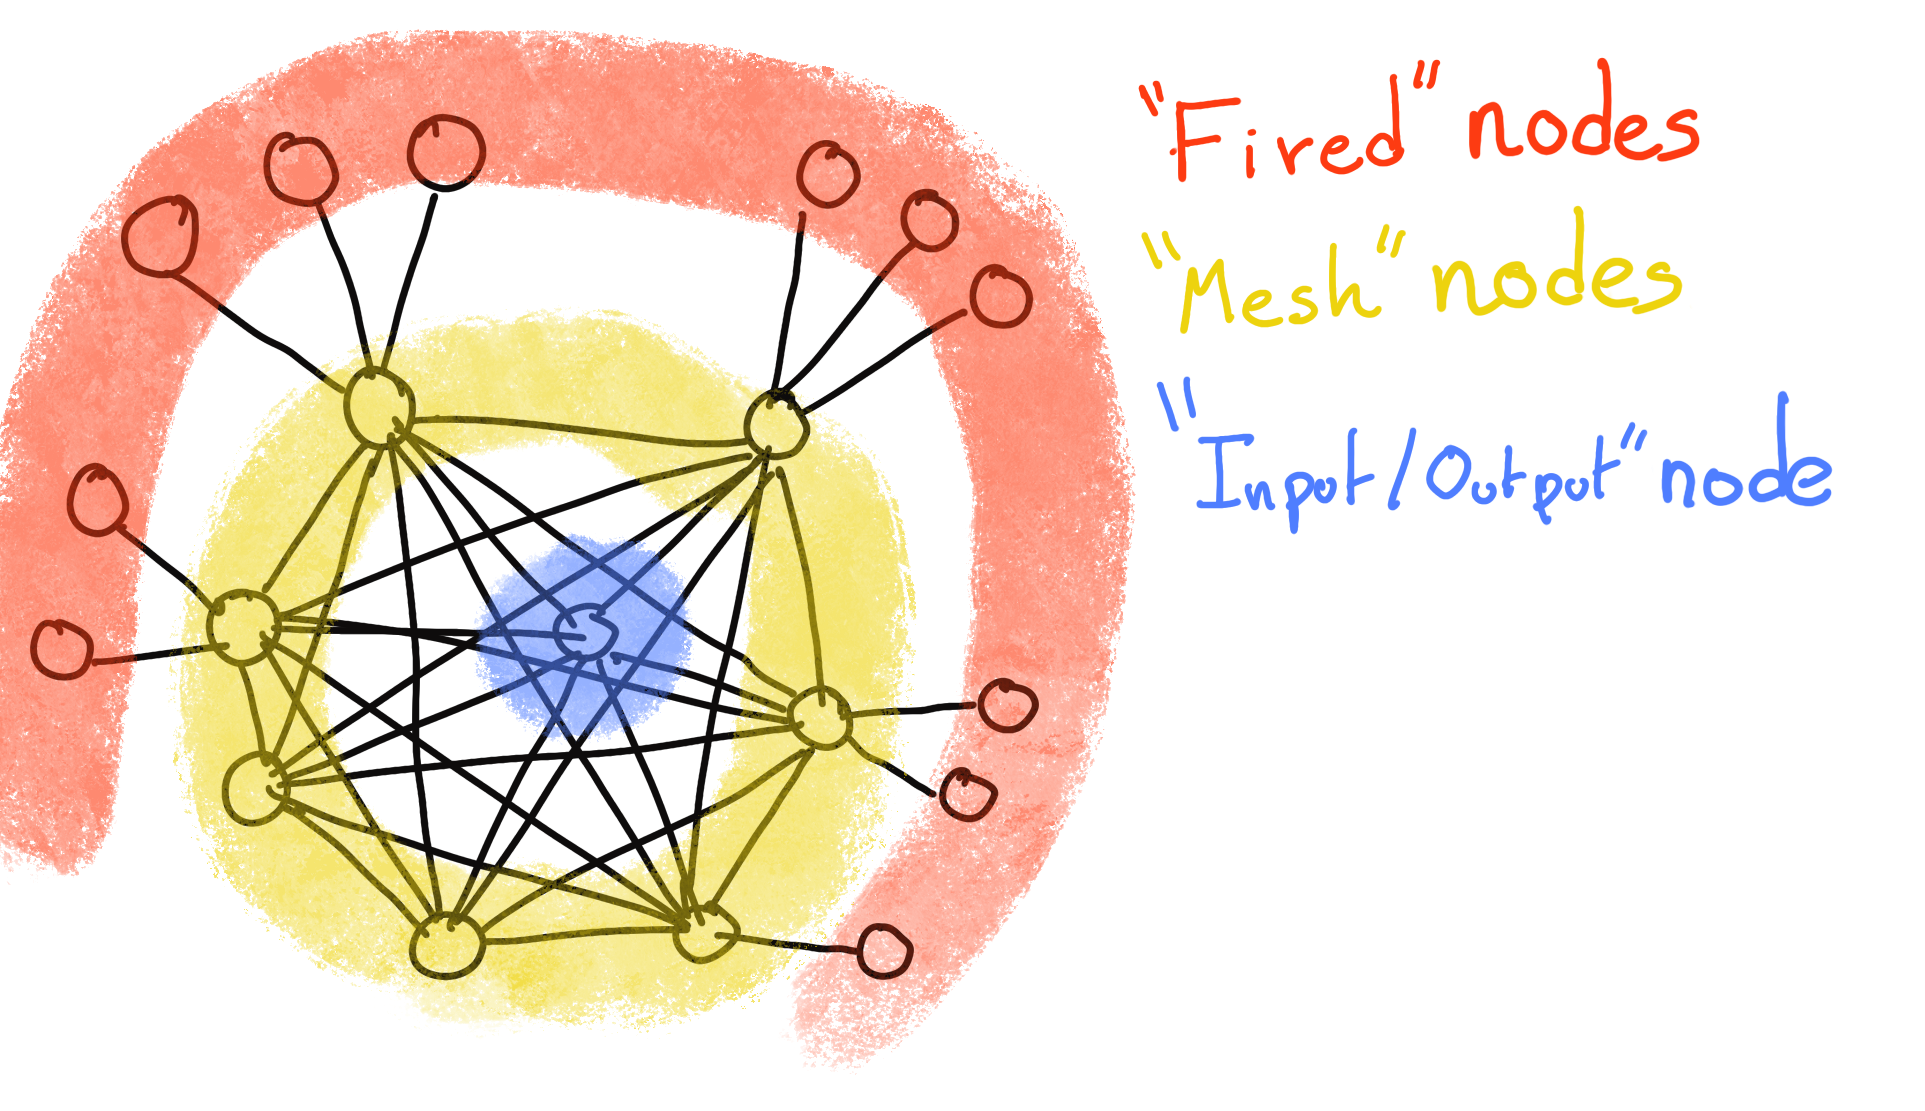
\includegraphics[width=\linewidth]{images/jgnn/nodes_schema.png}
    \caption{Illustration of the different nodes in our graphs and their relations.}
    \label{fig:jgnn:node_schema}
  \end{subfigure}
  \hfill
  \begin{subfigure}[t]{0.39\linewidth}
    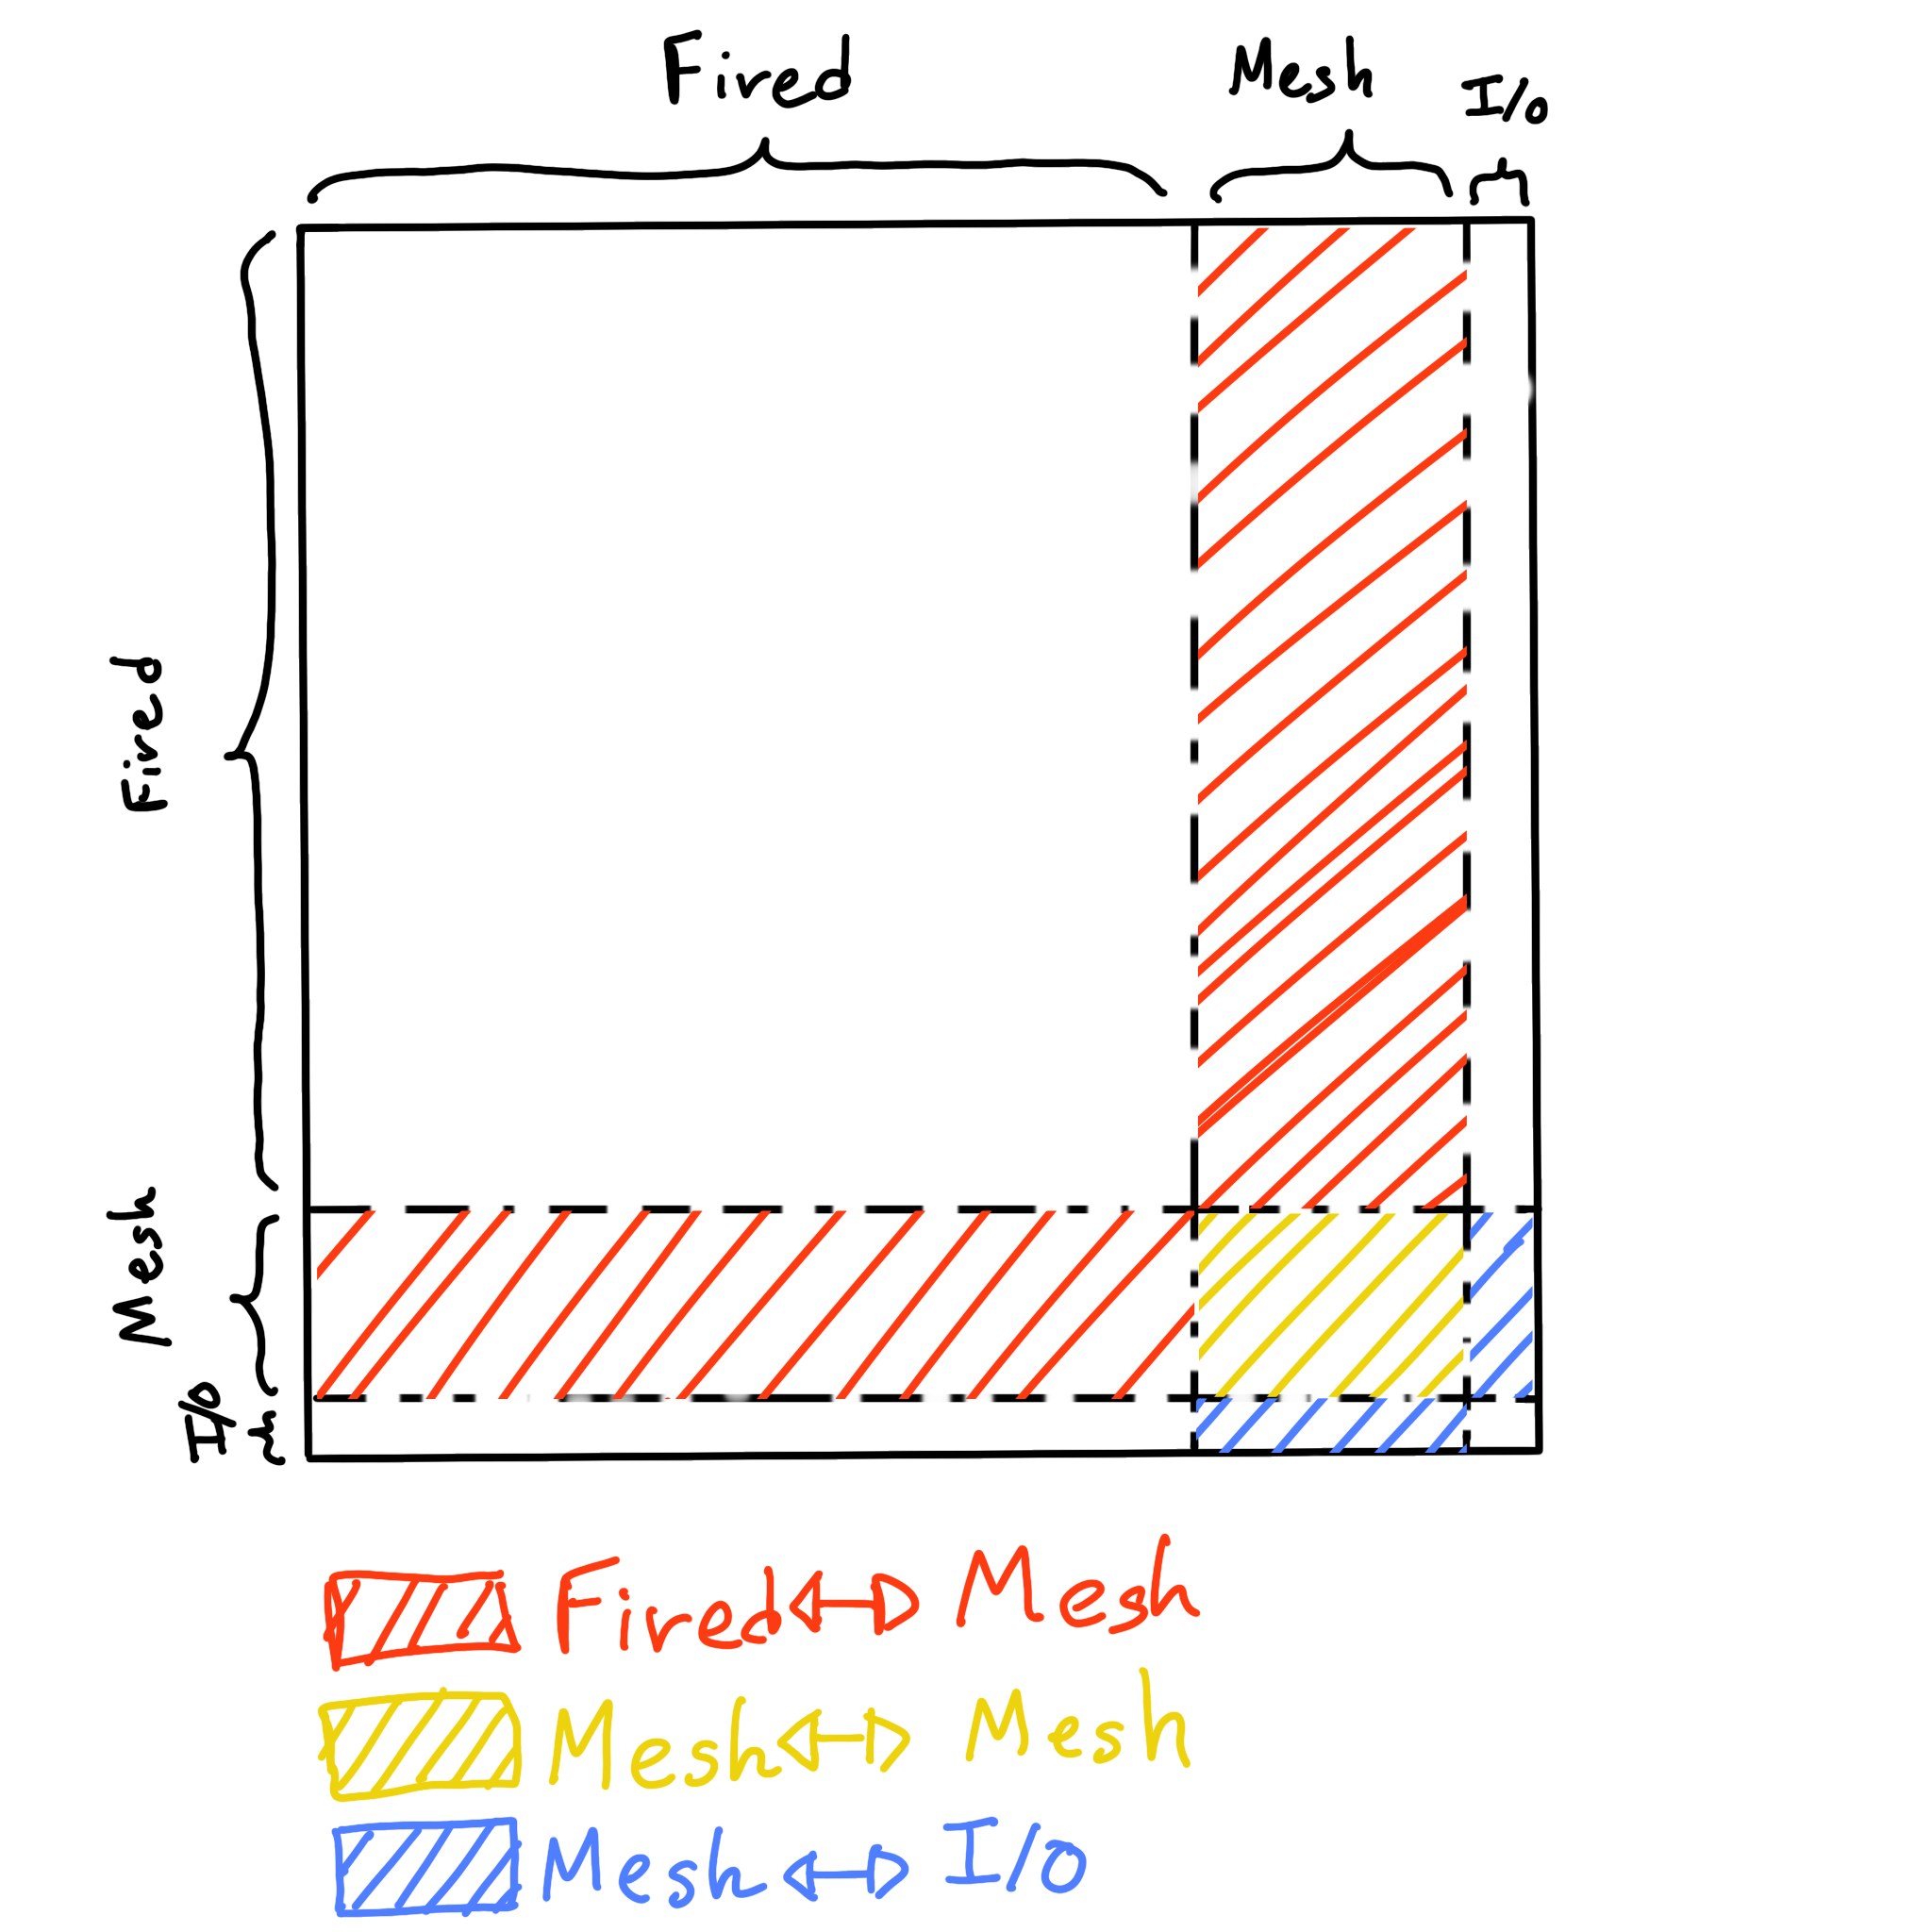
\includegraphics[width=\linewidth]{images/jgnn/adjacency_mat.png}
    \caption{Illustration of what a dense adjacency matrix would looks like and the part we are really interested in. Because Fired $\rightarrow$ Mesh and Mesh $\rightarrow$ I/O relations are undirected, we only consider in practice the top right part of the matrix for those relations.}
    \label{fig:jgnn:adj}
  \end{subfigure}
  \caption{}
\end{figure}

The mesh segmentation is following the Healpix segmentation \cite{gorski_healpix_2005}. This segmentation offer the advantage that almost each mesh have the same number of direct neighbours and it guarantee that each mesh represent the same extent of the detector surface. The segmentation can be infinitely subdivided to provide smaller and smaller pixels. The number of pixel follow the order $n$ with $N_{pix} = 12 \cdot 4^n$. This segmentation is illustrated in Figure \ref{fig:jgnn:healpix}. To keep the number of mesh small, we use the segmentation of order 2, $N_{pix} = 12 \cdot 4^2 = 192$.

\begin{figure}
  \centering
  \begin{subfigure}[t]{0.48\linewidth}
    \centering
    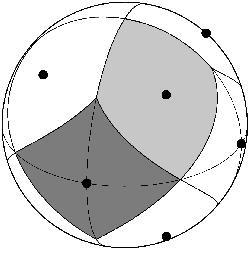
\includegraphics[width=0.5\linewidth]{images/jgnn/healpix_0.jpg}
  \end{subfigure}
  \hfill
  \begin{subfigure}[t]{0.48\linewidth}
    \centering
    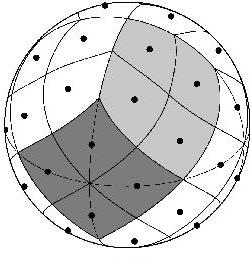
\includegraphics[width=0.5\linewidth]{images/jgnn/healpix_1.jpg}
  \end{subfigure}
  \caption{Illustration of the Healpix segmentation. \textbf{On the left:} A segmentation of order 0. \textbf{On the right:} A segmentation of order 1}
  \label{fig:jgnn:healpix}
\end{figure}

We decided on having the different kind of nodes {\color{Dandelion} mesh (M)}, {\color{red} fired (F)} and {\color{blue} I/O} have different set of features. The features used in the graph are presented in tables \ref{tab:jgnn:node_feat} and \ref{tab:jgnn:edge_feat}. Most of the features are low level informations such as the charge or time information but we include some high order features such as
\begin{enumerate}
  \item $P^h_l$: Is the normalized power of the $l$th spherical harmonic. For more details about spherical harmonics in JUNO, see annex \ref{sec:annex:jgnn:harms}.
  \item $\mathbb{A}$ and $\mathbb{B}$ are informations that are related the likeliness of the interaction vertex to be on the segment between the center of two meshes.
    \begin{align}
      \mathbb{A}_{ij} &= (\vec{j} - \vec{i})\cdot\frac{l_1}{D_{ij}} + \vec{i} \\
      \mathbb{B}_{ij} &= \frac{Q_i}{Q_j} \bigg(\frac{l_2}{l_1}\bigg)^2 \\
      l_1 &= \frac{1}{2}(D_{ij} - \Delta t \frac{c}{n}) \\
      l_2 &= \frac{1}{2}(D_{ij} + \Delta t \frac{c}{n})
    \end{align}
    where $\vec{i}$ is the position vector of the mesh $i$, $D_{ij}$ is the distance between the center of the meshes $i$ and $j$, $Q_i$ the sum of charges on the mesh $i$, $\Delta t = t_i - t_j$ where $t_i$ the earliest time on the mesh $i$ and $n$ the optical index of the LS. $\mathbb{A}$ is the vertex between center of meshes distance ratio between $i$ and $j$ based on the time information. For $\mathbb{B}$, the charge ratio evolve with the square of the distance, so the mesh couple with the smallest $\mathbb{B}$ should be the one with the interaction vertex between its two center.
\end{enumerate}

\begin{table}[ht]
  \centering
  \begin{tabular}{|c|c|c|}
    \hline
    Fired & Mesh & I/O \\
    \hline \hline
    $Q$ & $\langle Q_m \rangle$ & $\langle X \rangle$ \\
    $t$ & $\sigma Q_m$ & $\langle Y \rangle$ \\
    $x$ & $\mathrm{min}(t_m)$ & $\langle Z \rangle$ \\
    $y$ & $\mathrm{max}(t_m)$ & $\sum Q$ \\
    LPMT/SPMT: 1/-1 & $\sigma t_m$ & $P^h_l; ~ l \in [0,8]$ \\
            & $X_m$ & \\
             & $Y_m$ & \\
             & $Z_m$ & \\
    \hline
  \end{tabular}
  \caption{Features on the nodes of the graph. All charge are in [nPE], time in [ns] and position in [m]. \\
  $Q$ and $t$ are the reconstructed charge and time of the hit PMTs. $(x,y,z)$ is the position of the PMTs and the last parameter represent the type of the PMT. It's 1 for LPMT and -1 for SPMT \\
  $Q_m$ and $t_m$ is the set of charges and time of the PMT belonging the mesh $m$. $(X_m, Y_m, Z_m)$ i the position of the center of the geometric region represented by the mesh $m$ \\
  $(\langle X \rangle, \langle Y \rangle, \langle Z \rangle)$ is the position of the charge barycenter, $\sum Q$ the sum of the collected charge in the detector and $P^h_l$ is the relative power of the $l$th harmonic. See annex \ref{sec:annex:jgnn:harms} for details.}
  \label{tab:jgnn:node_feat}
\end{table}


\begin{table}
  \centering
  \begin{tabular}{|c|c|c|}
    \hline
    Fired $\rightarrow$ Mesh & Mesh ($m1$) $\rightarrow$ Mesh ($m2$) & Mesh $\rightarrow$ I/O \\
    \hline \hline
    $x - X_m$ & $X_{m1} - X_{m2}$ & $\langle X \rangle - X_m$ \\
    $y - Y_m$ & $Y_{m1} - Y_{m2}$ & $\langle Y \rangle - Y_m$ \\
    $z - Z_m$ & $Z_{m1} - Z_{m2}$ & $\langle Z \rangle - Z_m$ \\
    $t - \mathrm{min}(t_m)$ & $\mathrm{min}(t_{m1}) - \mathrm{min}(t_{m2})$ & $\sum Q_m / \sum Q$ \\
    $Q / \sum Q_m$ & $\frac{\langle Q_{m1} \rangle - \langle Q_{m2} \rangle}{\langle Q_{m1} \rangle + \langle Q_{m2} \rangle}$ & $\langle t_m \rangle$ \\
     & $D^{-1}_{m1 \rightarrow m2}$ & \\
     & $\mathbb{A}$ & \\
     & $\mathbb{B}$ & \\
    \hline
  \end{tabular}
  \caption{Features on the edges on the graph. It use the same notation as in table \ref{tab:jgnn:node_feat}. $D^{-1}_{m1 \rightarrow m2}$ is the inverse of the distance between the mesh $m1$ and the mesh $m2$. The features $\mathbb{A}$ and $\mathbb{B}$ are detailed in Section \ref{sec:jgnn:data}}
  \label{tab:jgnn:edge_feat}

\end{table}

Since our different nodes do not have the same number of features, they exist in distinct spaces. Traditional graph neural networks only handle homogeneous graphs, where the nodes and edges have the same number of features at each layer. Therefore, the libraries and publicly available algorithms we found were not suited to our needs. As a result, we had to develop and implement a custom message-passing algorithm capable of handling our heterogeneous graph.

\section{Message passing algorithm}
\label{sec:jgnn:mpa}
%\begin{itemize}
%  \item Need one message passing algorithm per connection (f->m, m->f, m->m, n->io, io->m)
%  \item Allow to select part of the adjacency matrix (see notes)
%  \item Explain message passing layer that was developed
%  \item Reimplementation in C++ using torch framework
%  \item C++ allow also for on the fly data transformation from raw file and minutieuse memory management
%  \item Not updating the edge for the sake of technical simplicity: Commplicated to identify an edge feature from the above algorithm
%\end{itemize}
The message passing algorithm define the way the GNN will compute and update its graph. As it is detailled in Section \ref{sec:ml:gnn}, the message-passing algorithm allows each node in the graph to update its features based on information from its neighboring nodes. This update process enables the network to propagate information through the graph, allowing nodes to gradually integrate knowledge about the entire detector. This step is crucial for ensuring that each node can take into account not only its local neighborhood but also the broader context of the event.

As introduced in previous section and in the tables \ref{tab:jgnn:node_feat} and \ref{tab:jgnn:edge_feat}, our graphs nodes and edges will have different number of features depending on their nature, meaning that we cannot have a single message passing function. We thus need to define a message passing function for each transition inside or outside a family. Using the notation presented in Section \ref{sec:ml:gnn}:
\begin{equation}
  \label{eq:jgnn:gen_mp}
  n_i^{k+1} = \phi_u (n_i^k, \Box_j \phi_m(n_i^k, n_j^k, e^k_{ij})); ~ n_j \in \mathcal{N}'_i
\end{equation}
and denoting the mesh nodes $M$, the fired nodes $F$ and the I/O node $IO$, we need to define
\begin{align*}
  \phi_{u; F\rightarrow M}  ~;~ &\phi_{m; F\rightarrow M} \\
  \phi_{u; M\rightarrow F}  ~;~ &\phi_{m; M\rightarrow F} \\
  \phi_{u; M\rightarrow M}  ~;~ &\phi_{m; M\rightarrow M} \\
  \phi_{u; M\rightarrow IO} ~;~ &\phi_{m; M\rightarrow IO} \\
  \phi_{u; IO\rightarrow M} ~;~ &\phi_{m; IO\rightarrow M}
\end{align*}
to update the nodes after each layers. Following the illustration in Figure \ref{fig:jgnn:mp_ill}, for each transition between families or inside a family we need an aggregation, a message and an update function. For the aggregation, we use the sum. We use the same, simple, formalism for every $\phi_u$:
\begin{equation}
  \label{eq:jgnn:custom_mp}
  \phi_u \equiv I^{n'}_{i'} = I^n_i A_{i',e}^{i} W_n^{e,n'} + I^n_i S^{n'}_{n} + B^{n'}
\end{equation}
using the Einstein summation notation. The second order tensor, or matrix, $I^{n}_i$ is holding the nodes informations with $i$ the node index and $n$ the feature index. $n$ represent the features of the previous layer and $n'$ the features of this layer.

$A_{i',e}^{i}$ is the adjacency tensor, discussed in the previous section, representing the edges between the node $i'$ and the node $i$, each edges holding the features indexed by $e$. If the edge does not exist, the features are set to 0. This choice is justified by the linearity of the operation in equation \ref{eq:jgnn:custom_mp} : whatever the weights, when multiplied by 0 the results is 0 and the sum result is unchanged.

The learnable parameters are composed of:
\begin{itemize}
  \item The third order tensor $W_n^{e,n'}$ which represent the passage from the previous combined feature space between the node and the edge features $n \otimes e$, the previous layer, to the current space $n'$, this layer.
  \item The first order tensor $B^{n'}$ which is a learnable bias on the new features $n'$.
  \item The second order tensor $S^{n'}_n$, which can be viewed as a self loop relation where the node update itself based on the previous layer informations, going from the previous space $n$ to the current space $n'$.
\end{itemize}

If a node have neighbours in different families, the different $IAW$ coming from the different families are summed.
\begin{equation}
  \label{eq:jgnn:multi_fam}
  I' = \sum_\mathcal{N} \bigg[ I_{\mathcal{N}}AW \bigg] + IS + B
\end{equation}
where $\mathcal{N}$ are the neighbouring family.
In our case, dropping the tensor indices and indexing by family for readability, we get
\begin{align}
  I_F' &= I_M A_{M \rightarrow F} W_{M \rightarrow F} + I_F S_F + B_F \\
  I_M' &= I_F A_{F \rightarrow M} W_{F \rightarrow M} + I_M A_{M \rightarrow M} W_{M \rightarrow M} + I_{IO} A_{IO \rightarrow M} W_{IO \rightarrow M} + I_M S_M + B_M \\
  I_{IO}' &= I_M A_{M \rightarrow IO} W_{IO \rightarrow M} + I_{IO} S_{IO} + B_{IO}
\end{align}

\begin{figure}
  \centering
  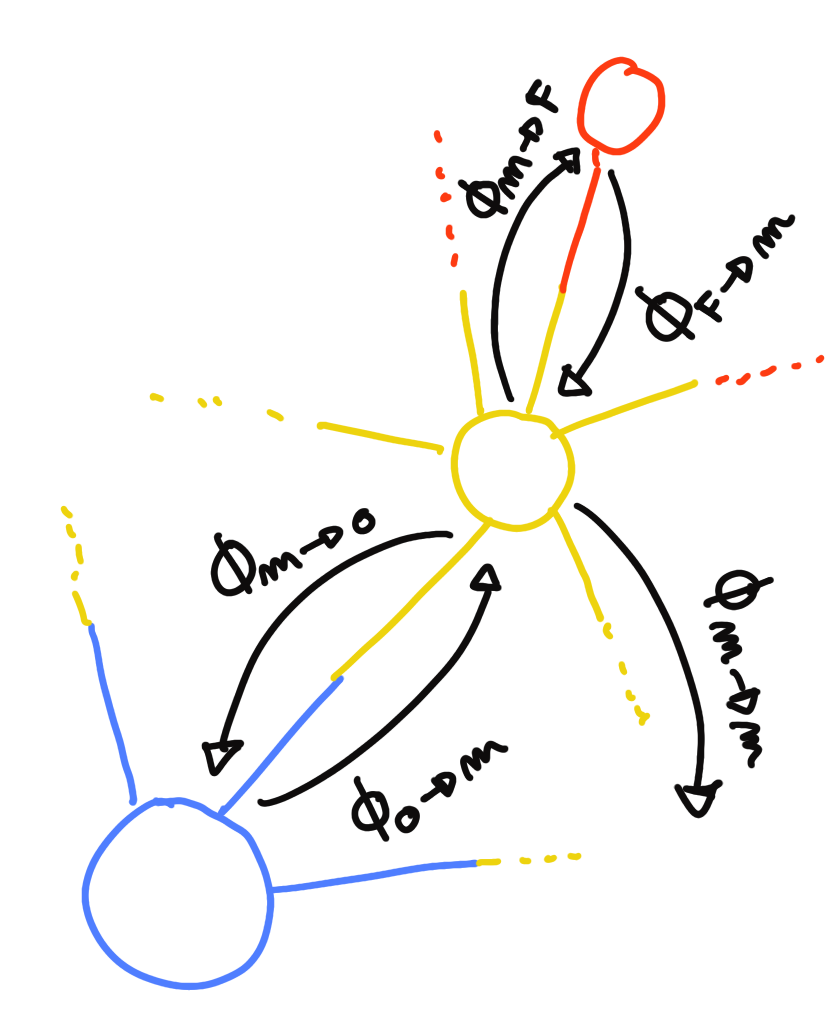
\includegraphics[height=5cm]{images/jgnn/mp_illus.png}
  \caption{Illustration of the different update function needed by our GNN}
  \label{fig:jgnn:mp_ill}
\end{figure}

We thus have a $S$, $W$ and $B$ for each of the $\phi_u$ function we defined above. The $IAW$ sum can be seen as the $\phi_m$ function and $IS+B$ as the second part of the $\phi_u$ function.
Eq \ref{eq:jgnn:gen_mp} gave the generic form of message passing : to update a node i, one first combines  informations from the surrounding nodes and edges and then combine the result ($\Box_j \phi_m$) with the current features of node i.
Many practical ways to combine can be tried. In our implementation of message passing (Eq. \ref{eq:jgnn:custom_mp} and \ref{eq:jgnn:multi_fam}) the latter combination is the simple sum of the former ( $IAW$, the equivalent of $\Box_j \phi_m$) with a linear combination of the current features of node i ($IS+B$).

Interestingly, the number on learnable weight in those layer is independent of the number of nodes in each family and depends solely on the number of features on the nodes and the edges.

The expression above only update the node features. We could update the edges, using the results of $\phi_m$ for example, but for technical simplicity we only update the nodes and keep the edges constant. Preserving the edges after each layers allow to share the adjacency matrix between all layers, saving memory and computing time.

This operation of message passing is the constituent of our message passing layers, designed in this work as \textit{JWGLayer}, each of them owning there own set of parameter $W$, $S$ and $B$. To those layers, we can adjoin an activation function such as $PReLU$
\begin{equation}
  I' = PReLU\bigg(\sum_\mathcal{N} \bigg[ I_{\mathcal{N}}AW \bigg] + IS + B \bigg)
\end{equation}


\section{Data}
%\begin{itemize}
%  \item Present the data (dataset)
%  \item Maybe show an example
%\end{itemize}


The dataset consists of 1M simulated positron events from the JUNO official simulation version J23.0.1-rc8.dc1. This version of the simulation incorporates both the physics of the detector and its electronics, ensuring that the events closely reflect real detector conditions. Importantly, this version includes advanced digitization and trigger modeling, making it suitable for testing the reconstruction capabilities of our GNN model. Those events are uniformly distributed in energy with $E_k \in [0, 9]$ MeV and distributed in the detector.

All the event are \textit{calib} level, with simulation of the physics, electronics, digitizations and triggers. 900k events will be used for the training, 50k for validation and loss monitoring and 50k for the results analysis in Section \ref{sec:jgnn:results}. Each events is between 2k and 12k fired PMTS, resulting in fired nodes being the largest family in our graphs in all circumstances as illustrated in Figure \ref{fig:jgnn:tot_hit_e}.

As expected, by comparing the scale between the Figure \ref{fig:jgnn:lpmt_hit_e} and \ref{fig:jgnn:spmt_hit_e} we see that the LPMT system is predominant in term of informations in our data. The number of PMT hits grow with energy but do not reach 0 for low energy event due to the dark noise contribution which seems to be around 1000 hits per event for the LPMT system (left limit of Figure \ref{fig:jgnn:lpmt_hit_e}) and around 15 hits per event for the SPMT system (left limit of Figure \ref{fig:jgnn:spmt_hit_e}) which is consistent with the results show in Section \ref{sec:jcnn:data}.

\begin{figure}[ht]
  \centering
  \begin{subfigure}[t]{0.32\linewidth}
    \centering
    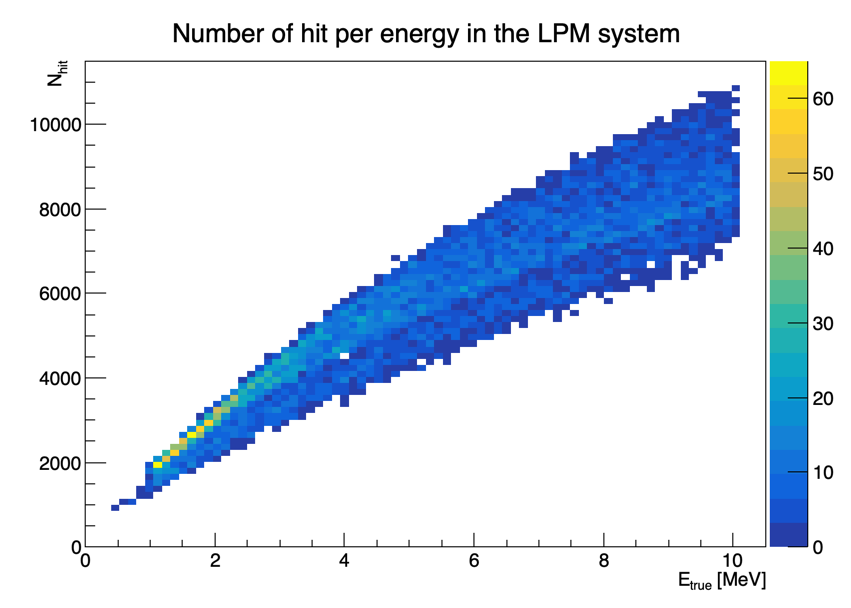
\includegraphics[width=\linewidth]{images/jgnn/lpmt_hit_e.png}
    \caption{}
    \label{fig:jgnn:lpmt_hit_e}
  \end{subfigure}
  \begin{subfigure}[t]{0.32\linewidth}
    \centering
    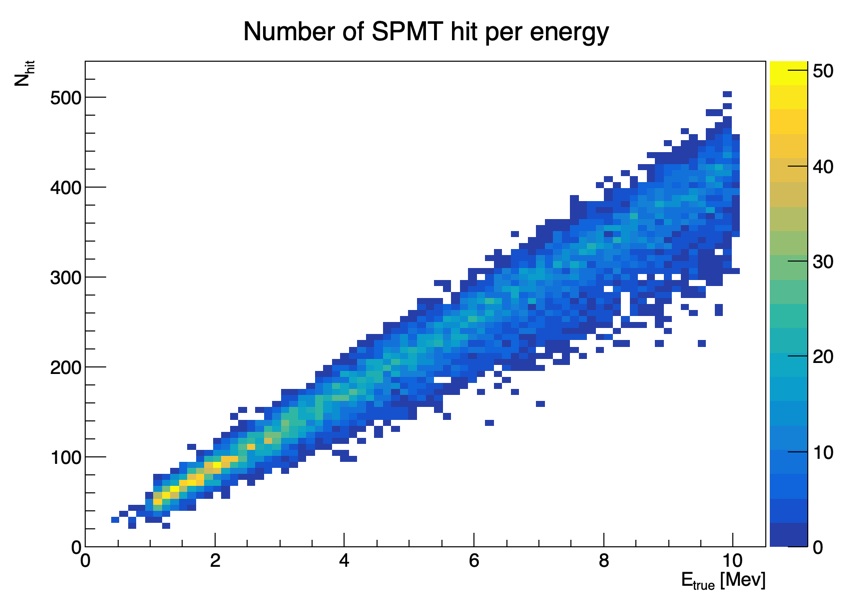
\includegraphics[width=\linewidth]{images/jgnn/spmt_hit_e.png}
    \caption{}
    \label{fig:jgnn:spmt_hit_e}
  \end{subfigure}
  \begin{subfigure}[t]{0.32\linewidth}
    \centering
    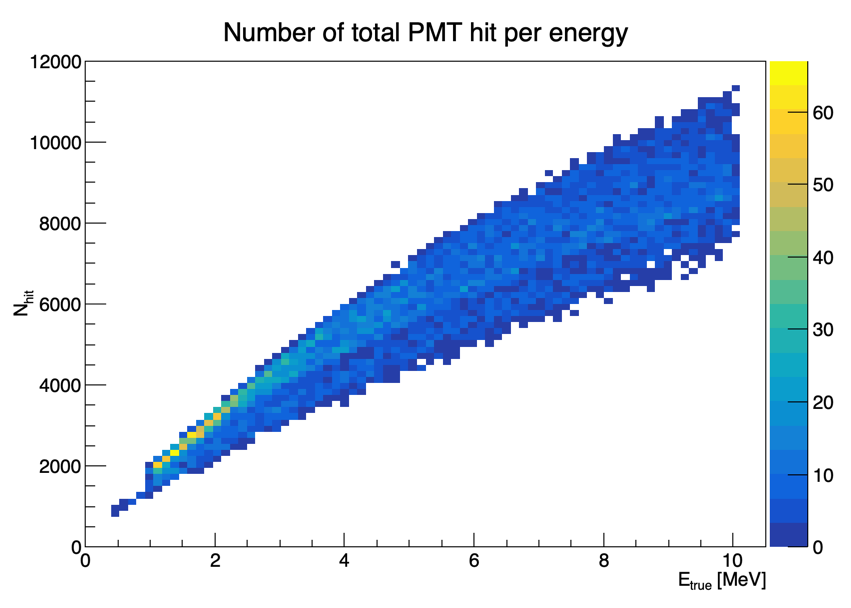
\includegraphics[width=\linewidth]{images/jgnn/tot_hit_e.png}
    \caption{}
    \label{fig:jgnn:tot_hit_e}
  \end{subfigure}
  \caption{Distribution of the number of hits depending on the energy. \textbf{On the right:} for the LPMT system. \textbf{In the middle :} for the SPMT system. \textbf{On the left: } For both system.}
\end{figure}

The structure seen in the distribution in Figure \ref{fig:jgnn:lpmt_hit_e} comes from the shape of the number of hits depending on the radius as shown in Figures \ref{fig:jgnn:lpmt_hit_r} and \ref{fig:jgnn:spmt_hit_r} where the number of hit decrease with radius. It is important to understand that this is not representative of the number of PE per event and the decrease in hits over the radius means that the PE are just more concentrated in a smaller number of PMTs.

\begin{figure}[ht]
  \centering
  \begin{subfigure}[t]{0.48\linewidth}
    \centering
    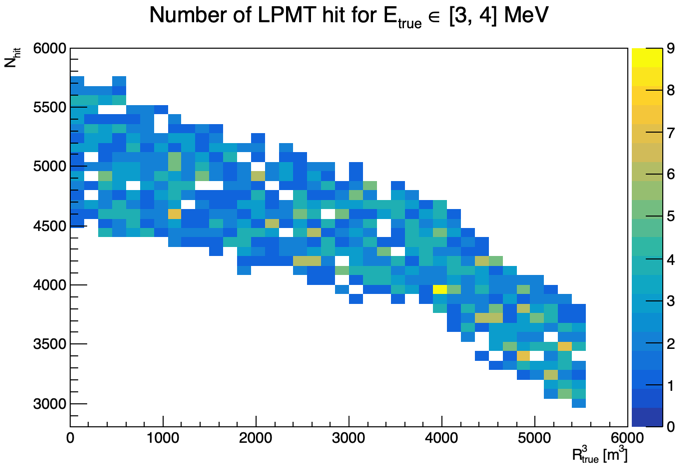
\includegraphics[width=\linewidth]{images/jgnn/lpmt_hit_r.png}
    \caption{}
    \label{fig:jgnn:lpmt_hit_r}
  \end{subfigure}
  \hfill
  \begin{subfigure}[t]{0.48\linewidth}
    \centering
    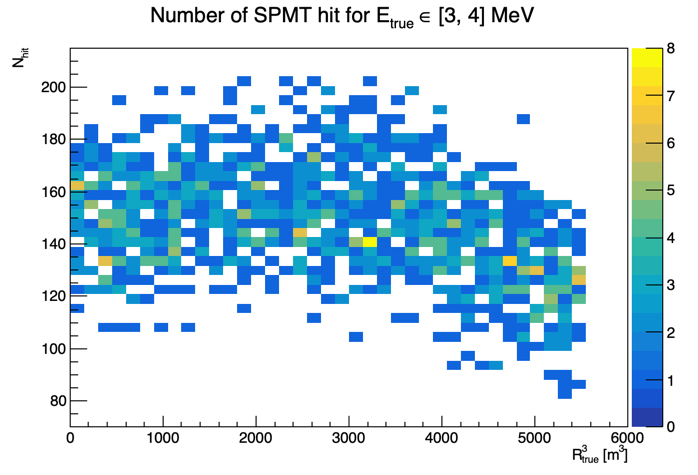
\includegraphics[width=\linewidth]{images/jgnn/spmt_hit_r.png}
    \caption{}
    \label{fig:jgnn:spmt_hit_r}
  \end{subfigure}
  \caption{Distribution of the number of hits depending on the radius. \textbf{On the right:} for the LPMT system. \textbf{On the right :} for the SPMT system. To prevent the superposition of structure of different scales we limit ourselves to the energy range $E_{true} \in [0, 9]$.}
\end{figure}

No quality cut is applied here, we rely only on the trigger system. It means that event that would not trigger are not present in the dataset but for events that triggered twice, it happens rarely, the two trigger are considered as two separate event.



\section{Model}
%\begin{itemize}
%  \item Present number of layers etc...
%  \item Discuss hyperparameters optimisation
%  \item Random search is not viable with the accessible hardware (too time consuming) -> 90h per trainng
%  \item By hand optimization -> around 70 iterations and tests.
%\end{itemize}

In this section, we discuss the different layers that compose the final version of the model. The number of layers, their dimensions, and their arrangement were fine-tuned through multiple iterations. As mentioned earlier, each JWGLayer is defined by the number of features on the nodes and edges of the output graph, assuming it takes as input the graph from the previous layer. For simplicity, when discussing a graph configuration, it will be presented as follow: \{ {\color{red} $N_{f}$},  {\color{Dandelion} $N_{m}$}, {\color{blue} $N_{IO}$}, $N_{f\rightarrow m}$, $N_{m \rightarrow m}$, $N_{m \rightarrow f}$ \} where
\begin{itemize}
  \item {\color{red} $N_{f}$} is the number of feature on the fired nodes.
  \item {\color{Dandelion} $N_{m}$} is the number of features on the mesh nodes.
  \item {\color{blue} $N_{IO}$} is the number of features on the I/O node.
  \item $N_{f\rightarrow m}$ is the number of features on the edges between the fired and mesh nodes.
  \item $N_{m \rightarrow m}$ is the number of features on the edges between two mesh nodes.
  \item $N_{m \rightarrow f}$ is the number of features on the edges between the mesh nodes and the I/O node.
\end{itemize}

Because we do not change the number of features on the edges, we can simplify the notation to \{{\color{red} $N_{f}$}, {\color{Dandelion} $N_{m}$}, {\color{blue} $N_{IO}$}\}. As an example, the input graph configuration, following the tables \ref{tab:jgnn:node_feat} and \ref{tab:jgnn:edge_feat} is \{{\color{red} 6}, {\color{Dandelion} 8}, {\color{blue} 13}, 5, 8, 5 \} or, without the edge features, \{{\color{red} 6}, {\color{Dandelion} 8}, {\color{blue} 13} \}.

The final version of the model, called JWGv8.4.0 is composed of
\begin{itemize}
  \item An JWGLayer, converting the input graph \{{\color{red} 6}, {\color{Dandelion} 8}, {\color{blue} 13} \} to \{ 64, 512, 2048 \} with a PReLU activation function.
  \item 3 resnet layers, each of them composed of
    \begin{enumerate}
      \item 2 JWG layers with a PReLU activation function. They do not change the dimension of the graph
      \item A sum layer that sums the features in the input graph with the one computed from the JWG layers
    \end{enumerate}
  \item A flatten layer that flatten the features of the I/O and mesh nodes in a vector.
  \item 2 fully connected layers of 2048 neurons with a PReLU activation function.
  \item 2 fully connected layers of 512 neurons with a PReLU activation function.
  \item A final, fully connected layer of 4 neurons acting as the output of the network.
\end{itemize}
A schematic of the model is presented in Figure \ref{fig:jgnn:model-schematic}.

We use the Mean Square Error (MSE) for the loss
\begin{equation}
  \mathcal{L} = (E_{rec} - E_{dep})^2 + (X_{rec} - X_{true})^2 + (Y_{rec} - Y_{true})^2 + (Z_{rec} - Z_{true})^2
\end{equation}
as it was the best resulting loss in Chapter \ref{sec:jcnn}.


\begin{figure}
  \centering
  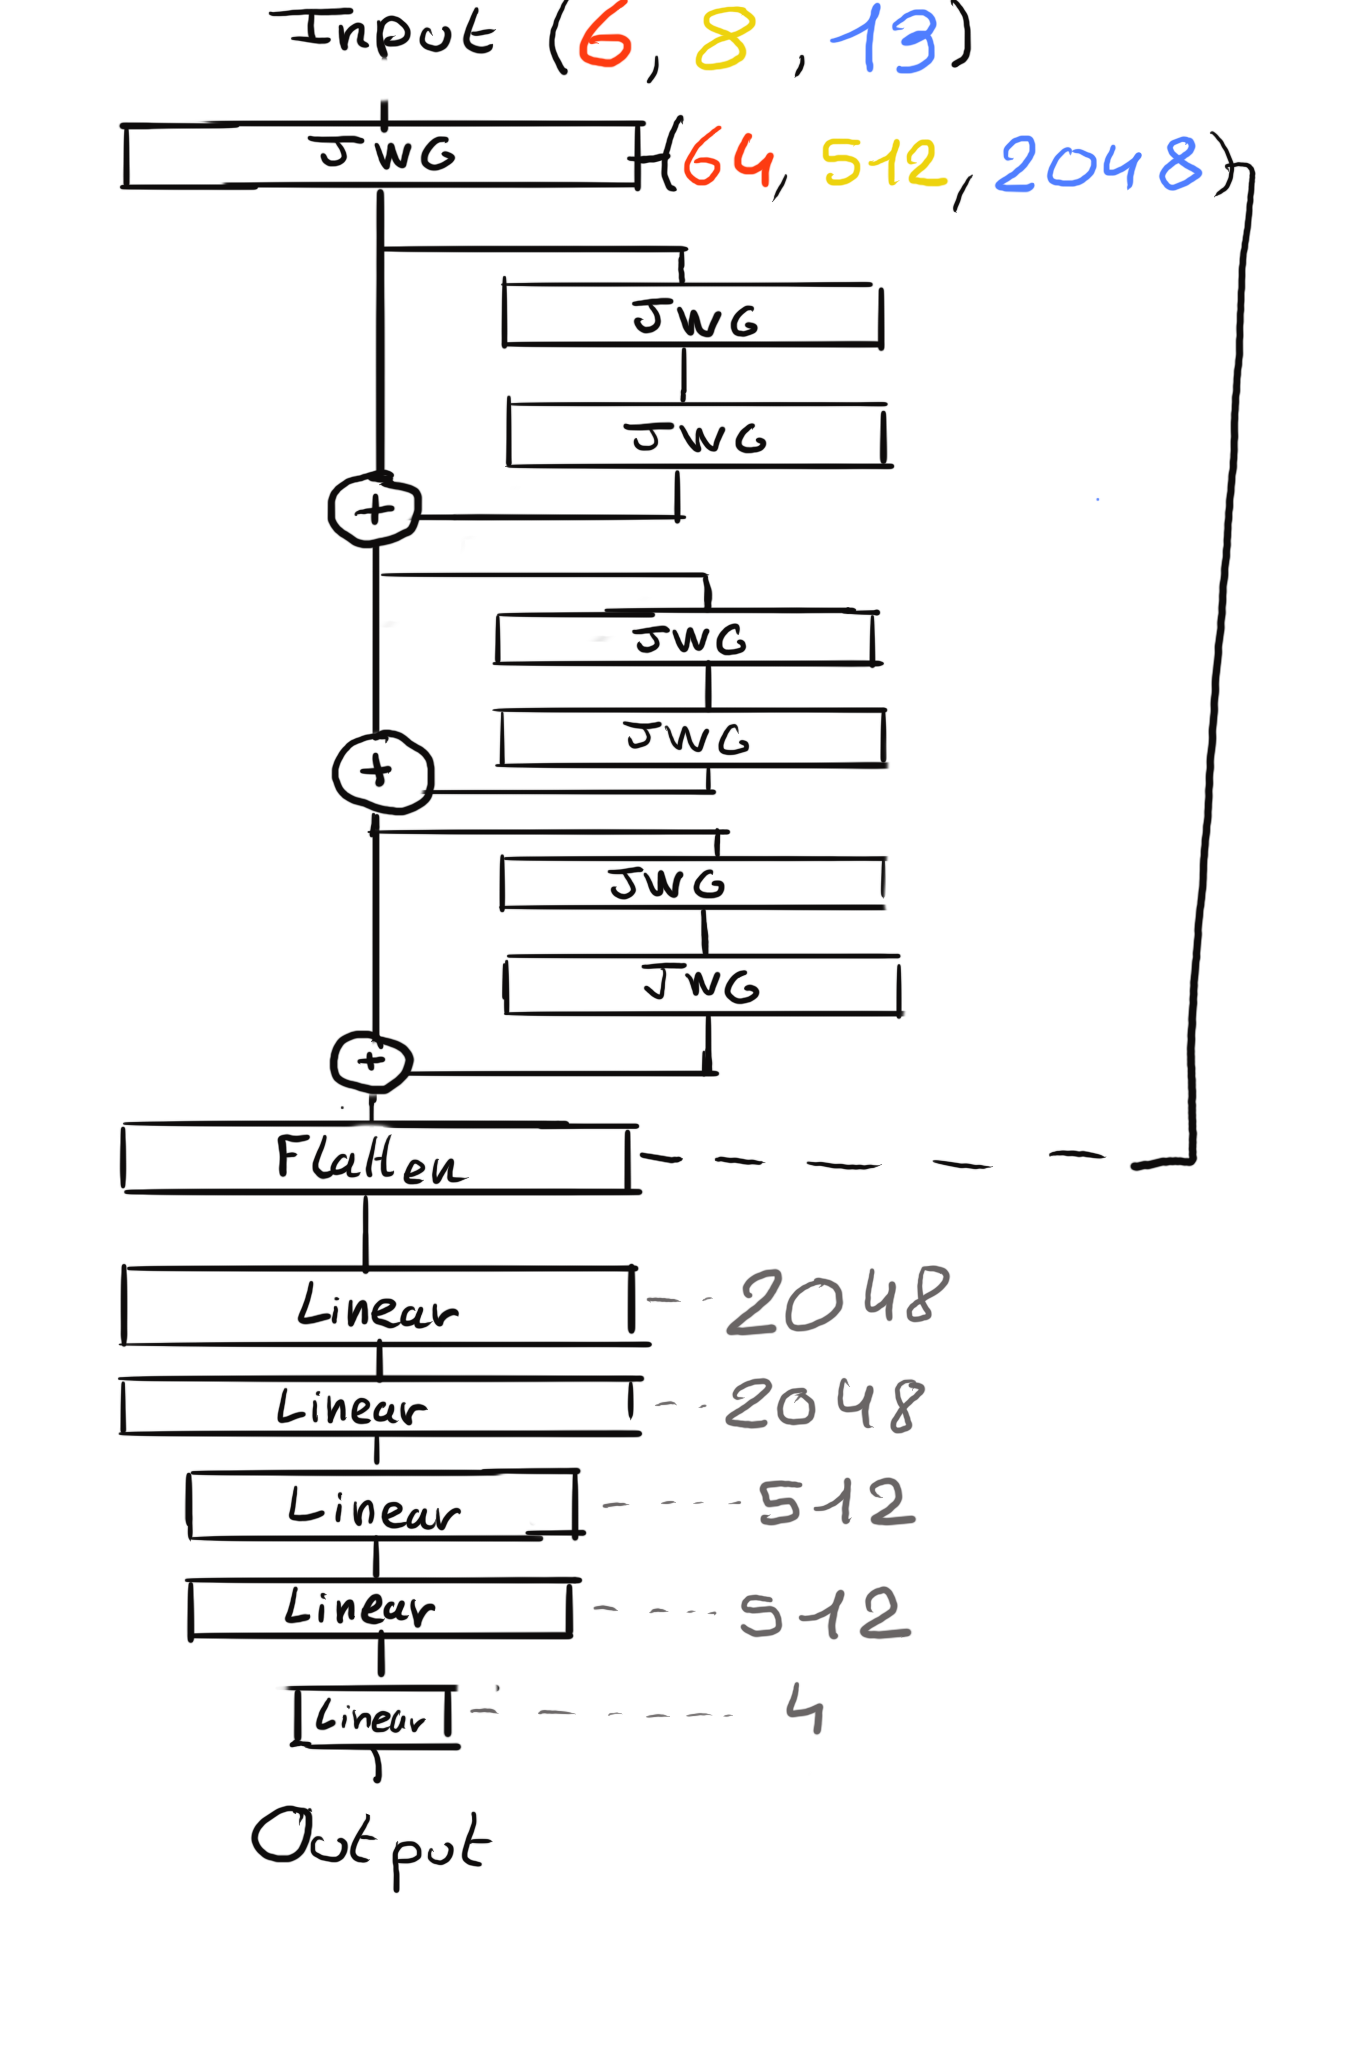
\includegraphics[height=12cm]{images/jgnn/jwgv8_4.png}
  \caption{Schema of the JWGv8.4.0 architecture, the colored triplet is the graph configuration after each JWG layers}
  \label{fig:jgnn:model-schematic}
\end{figure}


\section{Training}

The optimizer used for training is the Adam optimizer (see Section \ref{sec:ml:optim}) and default hyperparameters ($\beta_1= 0.9$, $\beta_2 = 0.999$ and $\epsilon = 1e-8$) with a learning rate $\lambda = $ 1e-8. The training last 200 epochs of 800 steps. We use a batch size of 32, the largest we can have with 40GB of GPU ram. The learning rate is constant during the first 20 epochs then exponentially decrease with a rate of 0.99. We save two set of parameters, the set of parameters the set that yield the lowest validation loss and the set of parameters at the end of the training. The validation is computed over a single batch.

\section{Optimization}

The GNN model presented in previous sections is the result of a long work of optimization. Indeed, the innovative architecture we propose left us with an infinity of possible configurations with no guidance from prior works in literature nor in JUNO.

In the end, more than 60 different configurations have been tested. This effort is illustrated on Figure \ref{fig:jgnn:histor}\footnote{Note that this figure was prepared on idealized data with no dark noise and perfect hit time determination.},
where the 40 configurations are compared in their ability to reconstruct the positron energy. Although all configurations share the fundamental principles we base our innovative architecture on (three different kinds of nodes and edges, usage of raw level features on some of them, usage of higher level data on others, division of JUNO's surface into regional pixels to form mesh nodes, the very large number of edges connected to each mesh node, etc.), performances can vary a lot between our first attempts (far beyond any acceptable energy resolution, and not even on this figure) and recent ones. Therefore: the precise way to choose hyperparameters mattered a lot, regardless of the relevance of the global architectural principles.

\begin{figure}
  \centering
  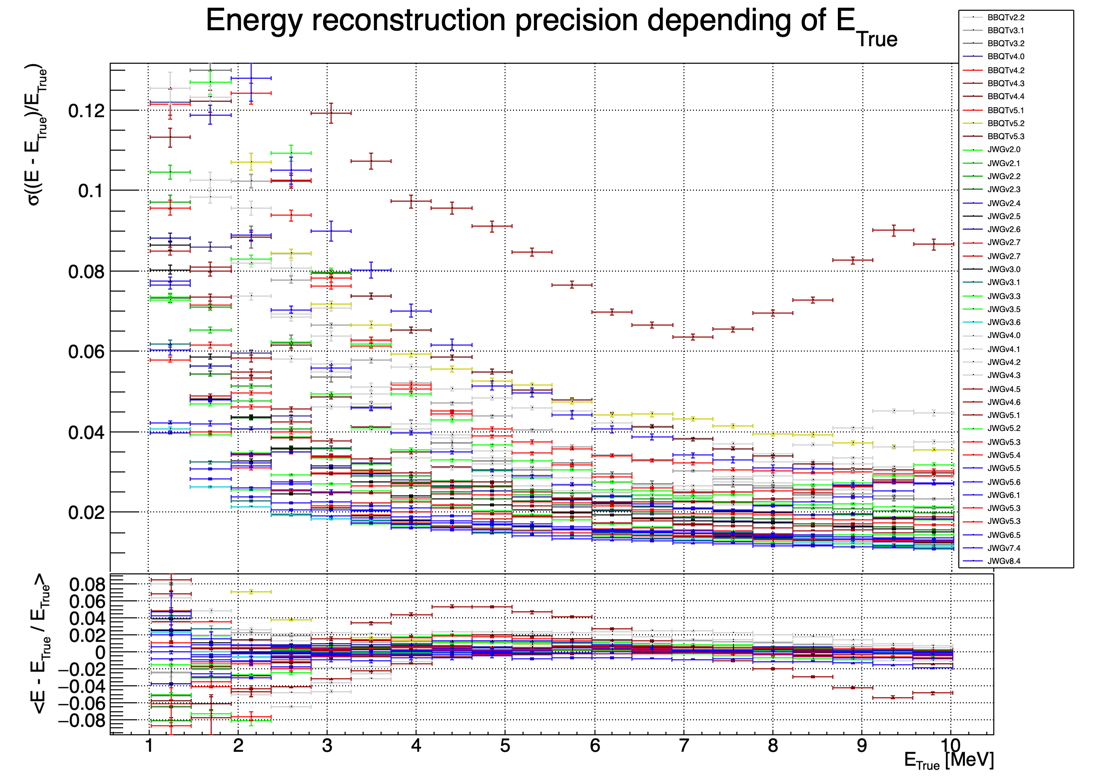
\includegraphics[height=6cm]{images/jgnn/GNN_Optimization_hist.png}
  \caption{Energy reconstruction depending on the true energy for samples of the different versions of the GNN}
  \label{fig:jgnn:histor}
\end{figure}

The spectacular improvement between early and later configurations also explains the length of this process : for long we hoped we would finally reach the classical performance, and it was tempting to test yet another configuration.

%Even the features on the graph went under investigation. With the addition of high level observables to the {\color{Dandelion} mesh} and {\color{blue} I/O} nodes and edge, there was too much possibility to test everything. We went with the decision to keep the raw observables in the {\color{red} fired} and for the higher order observables we tried to take the one that would be difficult for the NN to reconstruct or at least would need multiple layer to reproduce. Basically, because the operation in the JWGLayer are linear operation, any variables dependent on order  > 1 of the input would be candidates. This is why we introduce standard deviation, $\mathbb{A}$, $\mathbb{B}$ and $P^h_l$ for example.

\subsection{Software optimization}


A substantial effort was devoted to the data processing workflow. Transforming JUNO simulation outputs into graphs is a computationally expensive task. Furthermore, due to the ever-changing nature of the graph dimensions and features during optimization, preprocessing JUNO's files by precalculating the graphs and then reading them from files was not viable, as it would require a large amount of disk space to store events for each version of the graph.

Therefore, the software does not rely on preprocessed data and instead computes the observables, adjacency matrix, etc., during training. This data processing is performed in parallel on the CPU. The raw data comes from ROOT files produced by the collaboration software, and the Event Data Model (EDM), used internally by the collaboration \cite{li_design_2017}, had to be interfaced with our software, an interface that had to be maintained as the collaboration's software evolved. For the harmonic power calculation, we migrated from the Healpix library to Ducc0 \cite{reinecke_ducc0_2024} for more precise control over multithreading.

\subsection{Hyperparameters optimization}

The first kind of hyper-parameters that received a lot of effort concern the network's detailed architecture:
\begin{itemize}
  \item Message passing layers where originally not JWG layers, we started by using small FCDNN in place of $\phi_u$ and $\phi_m$. Due to low performances and memory consumption issues, we pivoted to the message passing algorithm presented in Section \ref{sec:jgnn:mpa}.

  \item The ResNet architecture was brought after issue with the gradient vanishing.

  \item The number of layers was varied between 5 and 12.

  \item The number of node features after each given message passing layer (64, 512, 2048 in the final version) was varied.

  \item The Final FCDNN after the message passing layers is not present in all versions.

  \item At some point, the PReLU activation function replaced the ReLU function.
\end{itemize}

\hfill

For some of them, software work was necessary. In any case, each configuration required a training of about 90h. Adding the analysis time necessary to the verification of its performance and the comparison with other versions, one understands the number of tests had to be limited.

Other hyperparameters were also tested :

\begin{itemize}

  \item The higher level variables described in Section \ref{sec:jgnn:data} (powers of various spherical harmonics, $\mathbb{A}$, $\mathbb{A}$, $(Q_{m1}-Q_{m2})/(Q_{m1}+Q_{m2})$ ) were added progressively. Notice that our choice to focus our search on this kind of variables is also due to the fact that JWGLayer involves linear operations. It is therefore difficult for such a network to propose variables of this kind among the node features learned layers after layers (i.e. it's difficult for the network to understand these variables are important, or only after many layers).


  \item Time allocated to training, the Learning Rate, the size of
    batches, etc.

  \item The number of pixels (ie of mesh nodes) was varied between 192 and 768.

  \item Several definitions  loss functions where tried. In particular, we tried some focussed only on the E resolution, only on the vertex resolution (R) or trying to optimize both.
\end{itemize}

\hfill

To make a long story short, each new configuration was the result of our reflections after having analysed the previous configurations, or  after having thought over again about JUNO's detailed response to energy deposits -- seeking for variables that could help the GNN.

Another, quite common, approach  was in principles possible : a random search. However, due to the extensive training time, up to 90h per training, the heavy memory consumption of the models that would often exceed the 20GB limit of the V100, this approach was not realistic in our case, though we were able to extend the memory limit to 40GB thanks to a local A100 GPU card available at Subatech.

\section{performance of the final version}
\label{sec:jgnn:results}


The reconstruction performance of ``JWGv8.4'' are presented in Figures \ref{fig:jgnn:results_nox_1}, \ref{fig:jgnn:results_nox_2}, \ref{fig:jgnn:results_nox_3} and compared to the ``Omilrec'' algorithm, the official IBD reconstruction algorithm in JUNO. Omilrec is based on the QTMLE reconstruction method that was presented in Section \ref{sec:juno:reco}.

This comparison required to use a consistent definition of $E_{true}$. This is not trivial since at JUNO, ML method reconstruct the true energy deposited by the positron+annihilation gammas (that's the target implemented in the loss function), while Omilrec, which is based on probabilities to observe a given number of PE in a given PMT, reconstruct the "visible energy". It reflects the total number of radiated and detectable scintillation or Cherenkov photons (and is subject to non linear effects like quenching).

The conversion we use to obtain comparable $E_{true}$ is explained in Appendix \ref{sec:annex:evis}.

On Figures \ref{fig:jgnn:results_nox_1} to \ref{fig:jgnn:results_nox_3}, we notice that the best GNN does not match the performance of the OMILREC algorithm. Generically, Energy resolution is 50\% worse, while the resolution on R is three times worse. Reconstruction biases are not better either with the GNN. We have tried to understand the origin of this limited performance.


%The reconstruction performance of ``JWGv8.4'' are presented in Figures \ref{fig:jgnn:results} and compared to the ``Omilrec'' algorithm, the official IBD reconstruction algorithm in JUNO. Omilrec is based on the QTMLE reconstruction method that was presented in Section \ref{sec:juno:reco}.
%
%We also present the results of the optimal variance combination of the two algorithm labelled as ``JWG 8.4 x Omilrec'' where the reconstructed target $\hat{theta}$ is the weighted sum of the result of the two estimator JWGv8.4 $\theta_J$ and Omilrec $\theta_O$.
%\begin{equation}
%  \hat{\theta} = \alpha \theta_J + (1 - \alpha) \theta_O; ~ \alpha \in [0, 1]
%\end{equation}
%For more details about the combination and the computation of $\alpha$, refer to annex \ref{sec:annex:jcnn:variance}.


\begin{figure}[ht]
  \centering
  \begin{subfigure}[t]{0.48\linewidth}
    \centering
    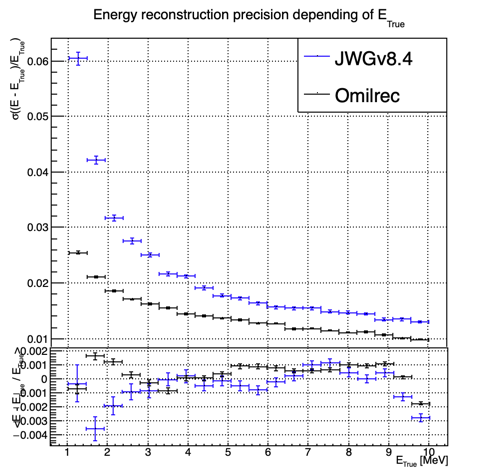
\includegraphics[width=\linewidth]{images/jgnn/MESBvET_nox.png}
    \caption{Resolution and bias of energy reconstruction vs energy}
    \label{fig:jgnn:MESBvETC_nox}
  \end{subfigure}
  \begin{subfigure}[t]{0.48\linewidth}
    \centering
    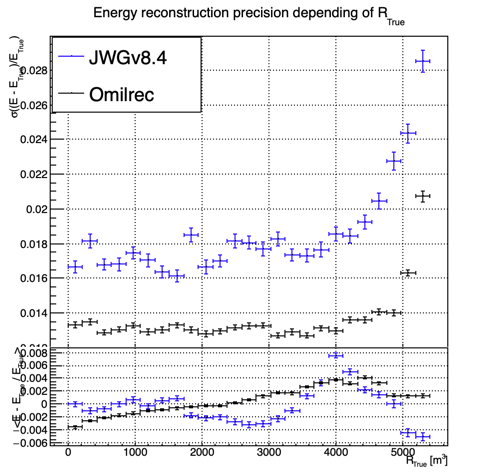
\includegraphics[width=\linewidth]{images/jgnn/MESBvRT_nox.png}
    \caption{Resolution and bias of energy reconstruction vs radius}
    \label{fig:jgnn:MESBvRTC_nox}
  \end{subfigure}
  \caption{Reconstruction performance of the Omilrec algorithm based on QTMLE presented in Section \ref{sec:juno:reco}, JWGv8.4 presented in this chapter. The top part of each plot is the resolution and the bottom part is the bias.}
  \label{fig:jgnn:results_nox_1}
\end{figure}
\begin{figure}[ht]
  \begin{subfigure}[t]{0.48\linewidth}
    \centering
    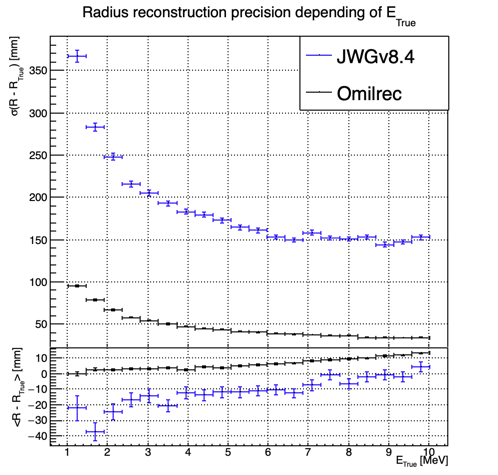
\includegraphics[width=\linewidth]{images/jgnn/MSBvTE_nox.png}
    \caption{Resolution and bias of radius reconstruction vs energy}
    \label{fig:jgnn:MSBvETC_nox}
  \end{subfigure}
  \begin{subfigure}[t]{0.48\linewidth}
    \centering
    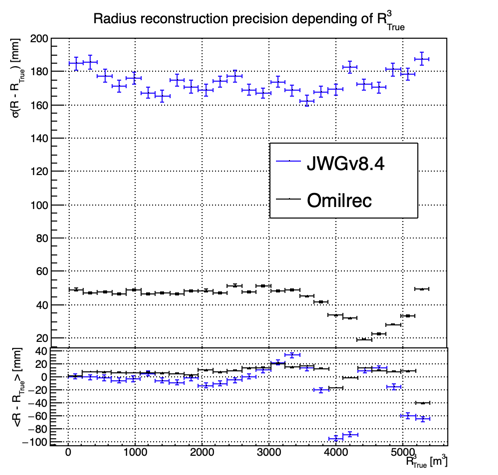
\includegraphics[width=\linewidth]{images/jgnn/MSBvRT_nox.png}
    \caption{Resolution and bias of radius reconstruction vs radius}
    \label{fig:jgnn:MSBvRTC_nox}
  \end{subfigure}
  \caption{Reconstruction performance of the Omilrec algorithm based on QTMLE presented in Section \ref{sec:juno:reco}, JWGv8.4 presented in this chapter. The top part of each plot is the resolution and the bottom part is the bias.}
  \label{fig:jgnn:results_nox_2}
\end{figure}
\begin{figure}
  \begin{subfigure}[t]{0.48\linewidth}
    \centering
    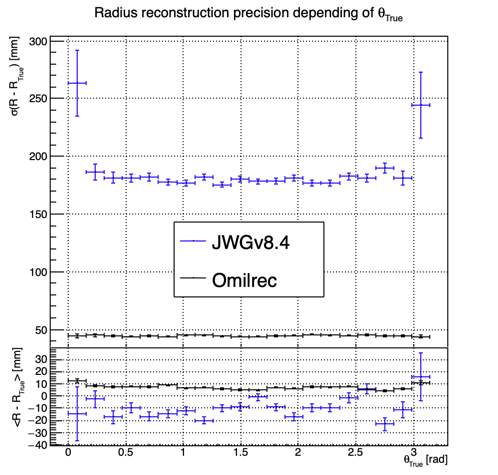
\includegraphics[width=\linewidth]{images/jgnn/MSBvTT_nox.png}
    \caption{Resolution and bias of radius reconstruction vs $\theta$}
    \label{fig:jgnn:MSBvTTC_nox}
  \end{subfigure}
  \begin{subfigure}[t]{0.48\linewidth}
    \centering
    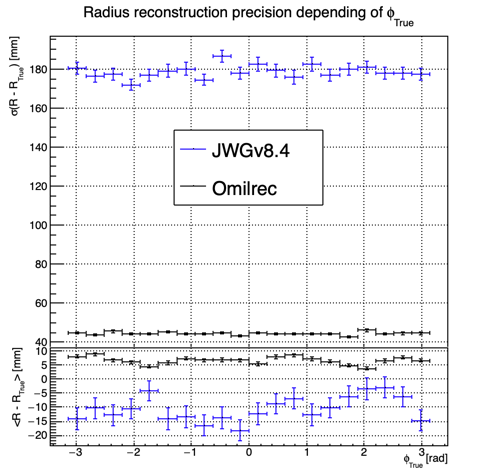
\includegraphics[width=\linewidth]{images/jgnn/MSBvPT_nox.png}
    \caption{Resolution and bias of radius reconstruction vs $\phi$}
    \label{fig:jgnn:MSBvPTC_nox}
  \end{subfigure}
  \caption{Reconstruction performance of the Omilrec algorithm based on QTMLE presented in Section \ref{sec:juno:reco}, JWGv8.4 presented in this chapter. The top part of each plot is the resolution and the bottom part is the bias.}
  \label{fig:jgnn:results_nox_3}
\end{figure}

The first action that can be carried out in this direction was to determine if some information used by OMILREC was not used properly by JWGv8.4. For that purpose, we used again the approach presented in Chapter \ref{sec:jcnn} (Sec \ref{sec:jcnn:combination} and annex \ref{sec:annex:jcnn:alpha} ) to combine JWGv8.4 and OMILREC. We observe on Figures \ref{fig:jgnn:results_1} and \ref{fig:jgnn:results_2} that this combination brings no sizeable improvement  of the best of the two combined methods. The combination remains very close to OMILREC alone. This is an indication that JWGv8.4 does not use informations that would be overlooked by OMILREC, and that on the contrary, that's JWGv8.4 that fails to use properly important informations.

%Overall, energy and radius resolutions are not on par with Omilrec. We see from the energy dependent energy resolution in fig \ref{fig:jgnn:MESBvETC} that our resolution is a bit more than twice the resolution of Omilrec and the combination brings no improvements. Same observation for the energy resolution depending on the radius.
%
%The radius resolution, presented in the Figures \ref{fig:jgnn:MSBvETC}, \ref{fig:jgnn:MSBvRTC}, \ref{fig:jgnn:MSBvTTC} and \ref{fig:jgnn:MSBvPTC} is much worse than the Omilrec one. This comes a bit as a surprise, as the energy reconstruction is dependent on the vertex reconstruction to correct for the non-uniformity and non-linearity effect. This mean that either the GNN could outperform the classical methods if the vertex was correctly reconstructed, or that somewhere the GNN reconstruct the vertex correctly but has trouble to formulate it in x,y,z coordinates on the latest layer.
%
%The GNN behaviours are close to Omilrec, indicating that the same information is used in the same way by both algorithms, just that the GNN seems to be less fine-tuned than Omilrec. If the precedent reasoning is true, it would mean that by adding more parameters, more layer or a higher pixelisation of the Healpix representation, the GNN could reach Omilrec performances.


\begin{figure}[ht]
  \centering
  \begin{subfigure}[t]{0.48\linewidth}
    \centering
    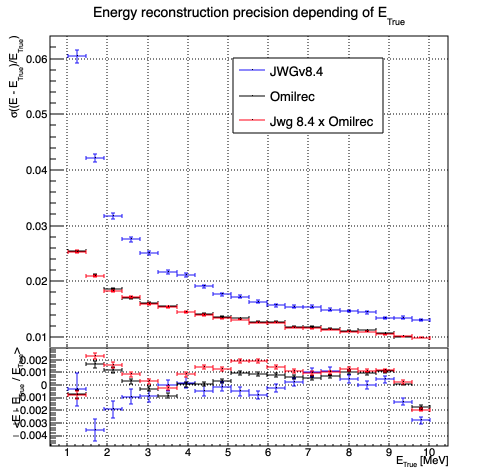
\includegraphics[width=\linewidth]{images/jgnn/MSBvTE.png}
    \caption{Resolution and bias of energy reconstruction vs energy}
    \label{fig:jgnn:MESBvETC}
  \end{subfigure}
  \begin{subfigure}[t]{0.48\linewidth}
    \centering
    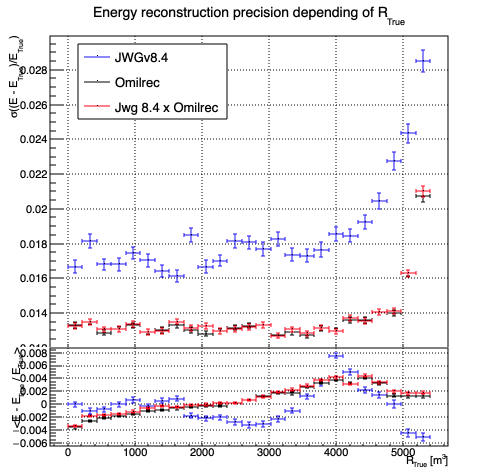
\includegraphics[width=\linewidth]{images/jgnn/MESBvRT.png}
    \caption{Resolution and bias of energy reconstruction vs radius}
    \label{fig:jgnn:MESBvRTC}
  \end{subfigure}
  \caption{Reconstruction performance of the Omilrec algorithm, JWGv8.4 and the combination between the two using the optimal variance estimator presented in annex \ref{sec:annex:jcnn:variance}. The top part of each plot is the resolution and the bottom part is the bias.}
  \label{fig:jgnn:results_1}
\end{figure}
\begin{figure}[ht]
  \begin{subfigure}[t]{0.48\linewidth}
    \centering
    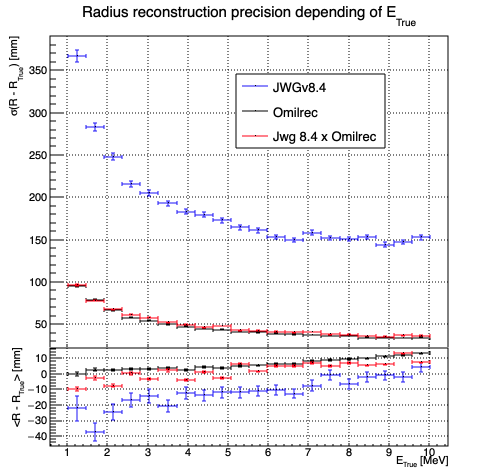
\includegraphics[width=\linewidth]{images/jgnn/MESBvET.png}
    \caption{Resolution and bias of radius reconstruction vs energy}
    \label{fig:jgnn:MSBvETC}
  \end{subfigure}
  \begin{subfigure}[t]{0.48\linewidth}
    \centering
    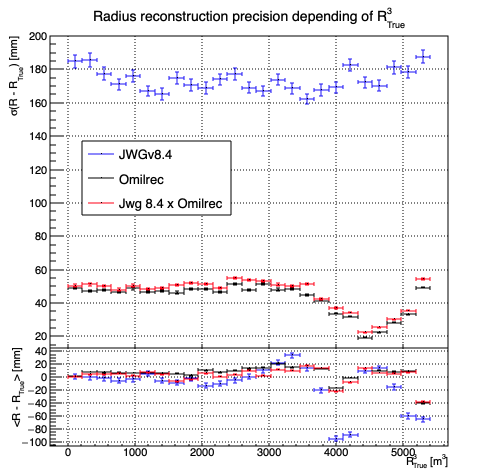
\includegraphics[width=\linewidth]{images/jgnn/MSBvRT.png}
    \caption{Resolution and bias of radius reconstruction vs radius}
    \label{fig:jgnn:MSBvRTC}
  \end{subfigure}
  \caption{Reconstruction performance of the Omilrec algorithm, JWGv8.4 and the combination between the two using the optimal variance estimator presented in annex \ref{sec:annex:jcnn:variance}. The top part of each plot is the resolution and the bottom part is the bias.}
  \label{fig:jgnn:results_2}
\end{figure}

The problem described above could be inherent to our GNN's original architecture. Discussions with JUNO's colleagues when these results were presented at the collaboration pointed to the role of PMT time information ($t$, in the $(Q,t)$ pairs we use as our algorithm input features). The thousands of values found in the \textit{fired} nodes might not be aggregated well enough when transmitted to the mesh nodes, causing a loss in the redundancy of this important information.

We tested this idea in several manners, described below.

\subsubsection{Finer granularity}

We tried to recover some redundancy by increasing the number of mesh nodes from 198 to 768. The improvement we observed was small, and did not allow to get close to OMILREC's performance.

To explore further in this direction, we would ideally try 3072 pixels (the next HEALPIX rank). However, this is not possible for our GNN due to hardware limitations, mainly the available GPU memory. Instead, we discussed the problem with Gilles Grasseau, calculus research engineer with whom we collaborate on the subject of ML reliability (see Chapter \ref{sec:janne}). In the framework of this activity, Gilles needs to develop reconstruction algorithms to be "attacked" by a prototype Adversarial NN. One of them is a pseudo-spherical CNN using oriented filters, called HCNN.


\begin{figure}[ht]
  \centering
  \begin{subfigure}[t]{0.48\linewidth}
    \centering
    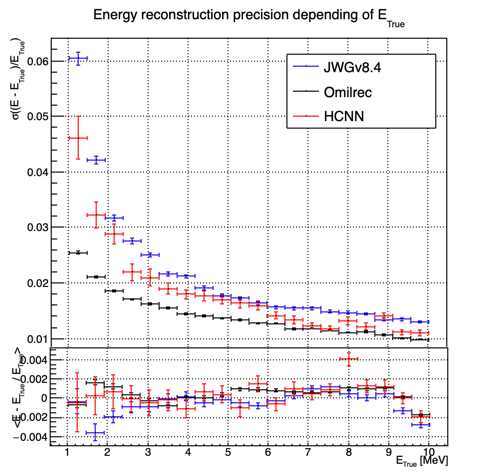
\includegraphics[width=\linewidth]{images/jgnn/hcnn/MESBvETC.png}
    \caption{Resolution and bias of energy reconstruction vs energy}
    \label{fig:jgnn:MESBvETC_hcnn}
  \end{subfigure}
  \begin{subfigure}[t]{0.48\linewidth}
    \centering
    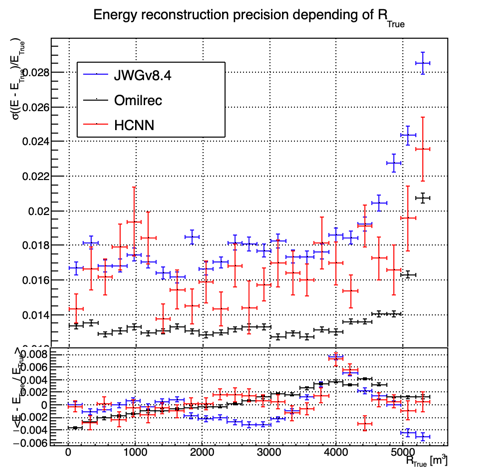
\includegraphics[width=\linewidth]{images/jgnn/hcnn/MESBvRTC.png}
    \caption{Resolution and bias of energy reconstruction vs radius}
    \label{fig:jgnn:MESBvRTC_hcnn}
  \end{subfigure}
  \caption{Reconstruction performance of the Omilrec algorithm based on QTMLE presented in Section \ref{sec:juno:reco}, JWGv8.4 presented in this chapter and the HCNN algorithm. The top part of each plot is the resolution and the bottom part is the bias.}
  \label{fig:jgnn:results_hcnn_1}
\end{figure}
\begin{figure}[ht]
  \centering
  \begin{subfigure}[t]{0.48\linewidth}
    \centering
    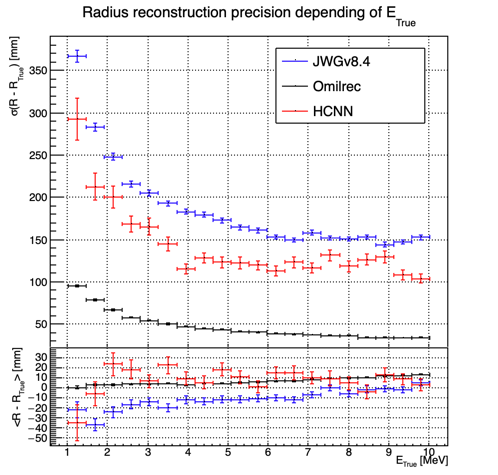
\includegraphics[width=\linewidth]{images/jgnn/hcnn/MSBvETC.png}
    \caption{Resolution and bias of radius reconstruction vs energy}
    \label{fig:jgnn:MSBvETC_hcnn}
  \end{subfigure}
  \begin{subfigure}[t]{0.48\linewidth}
    \centering
    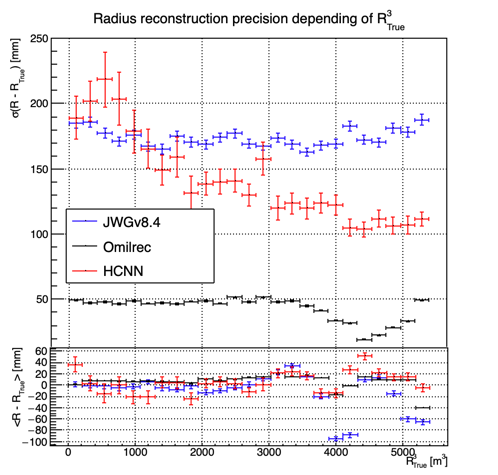
\includegraphics[width=\linewidth]{images/jgnn/hcnn/MSBvRTC.png}
    \caption{Resolution and bias of radius reconstruction vs radius}
    \label{fig:jgnn:MSBvRTC_hcnn}
  \end{subfigure}
  \caption{Reconstruction performance of the Omilrec algorithm based on QTMLE presented in Section \ref{sec:juno:reco}, JWGv8.4 presented in this chapter and the HCNN algorithm. The top part of each plot is the resolution and the bottom part is the bias.}
  \label{fig:jgnn:results_hcnn_2}
\end{figure}


%[comment ? JE te laisse l'écrire]
To produce its input image, this algorithms split the Sphere into 3072 pixels. Each channel of this image is an aggregation of the $(Q, t)$ values found in all the PMTs. The charge are summed and the lowest time is kept. The performance of this algorithm can be seen on Figures \ref{fig:jgnn:results_hcnn_1} and \ref{fig:jgnn:results_hcnn_2}, compared to OMILREC. With 3072 pixels, the performance of HCNN does not match that of OMILREC, but is closer to it than our GNN. The granularity of the pixels, and the way to summarize the individual PMTs information when going from 17000 LPMTs to only 3072 pixels indeed seems to play a role.

This is consistent with the results obtained by the first GNN tried at JUNO on reactor neutrinos (already described in Section \ref{sec:juno:ml}).
It used 3072 pixels, and also obtained an uncompetitive R reconstruction.

\subsubsection{Information reduction, from fired to Meshes}

The problem described above is somehow classical. ML algorithms, ideally, would start from the full information present in the detector, and learn to reduce it optimally.

In cases where only 3072 pixels can be used instead of the complete information from 17000 PMTs, one needs to understand how to combine the individual from the 5 or 6 PMT found in each pixel into pixel-level features, without loosing important information.

In the case of our GNN, we hoped that by connecting each mesh node to its corresponding 5 or 6 fired nodes, we could keep the full information. In reality, it seems that the message passing between fired and mesh does not work efficiently. When nodes are updated by the first (may be also by the subsequent) layer, the new mesh features might be dominated by the original features in the second column of tables \ref{tab:jgnn:node_feat}, themselves a simple version of aggregation.
Layer after layer, we might be limited to that level of time information, lacking time redundancy.

We have verified this by testing version of the GNN in which the link between fired and mesh was cut, or in which no time info was included among the fired nodes features. It had only a small effect
which seems to confirm a problem in the way the full information, from all the individual PMTs, is used by our GNN.

% (si cela peut-être quantifié, et on se fiche à ce niveau si c'est avec J21 plutôt que 23.,,),

\subsubsection{Possible improvements}


It appears that the network is unable to aggregate the timing information correctly. While this could be addressed by using a finer segmentation, with more mesh nodes, improvements might also arise from refining the message-passing algorithm. The algorithm presented in this thesis is still quite basic, relying on a simple linear combination of features. We have seen through examples in CNNs, GNNs, and other architectures, both in research and industry, that specializing the network — for instance, by incorporating convolutional filters — can lead to improvements that were previously unattainable with simpler FCDNNs. Applying this approach to the message-passing algorithm, by utilizing a GNN with a more advanced message-passing, could yield better results.

We could investigate alternative aggregation strategies, for example, by weighting the timing information more significantly during the message-passing phase. Additionally, testing a non-linear combination of features from fired to mesh nodes could help preserve more granular information. Another potential improvement would be to introduce attention mechanisms that dynamically assign more importance to relevant features in the fired nodes

Regarding the timing information, we provided high-level features, assuming this would assist the neural network in converging to the solution. However, by offering such information upfront, the GNN might be taking the ``easy'' path, settling for a local and broader minimum, rather than extracting the features that could lead to better performance.

If there are difficulties in transferring information between the fired and mesh nodes, it may stem from the way we connected the fired nodes to the mesh nodes. By linking the fired nodes within the same mesh, or even connecting the fired nodes of neighboring mesh nodes, the GNN might be able to construct more meaningful information.

Finally, by providing directly the PMT waveform to the GNN, in the fired nodes, we could search for even finer precision and results. An idea would be to specialise the message function $\phi_{m;F \rightarrow M}$ to be a 1D convolutional layer over the waveform. The resulting channels would be fed to the mesh nodes for their updates.

\section{Conclusion}

%\begin{itemize}
%  \item For now:
%  \item Not competitive
%  \item Aggregation on mesh nodes seems to loose informations
%  \item Maybe too complex ?
%  \item Next step would be to have the waveform dirrectly included
%\end{itemize}

%In this chapter, I present a proposition for a GNN architecture to reconstruct the energy and position of the prompt signal of an IBD interaction. The GNN is not competitive in terms of resolution with the more classical method Omilrec, which is the state of the art reconstruction method for IBD in the JUNO collaboration, but show encouraging results that could be exploited by going further in the optimisation of the hyper parameters. The message passing algorithm is still pretty naive and could probably be refined for JUNO's need.
%
%Another possible improvement is to find a way to increase the Healpix pixelisation. Through our different work on reconstruction and by looking at the different classical methods, it seems that the time information is crucial for the vertex reconstruction, and thus for the energy reconstruction. While we are keeping every raw informations about the fired PMTs, it is possible that the aggregation on mesh nodes could cause the information loss and it has been noticed that allowing more channels to the hidden layer mesh nodes improve the resolution. This observation can be compared to the convolutional GNN presented Section \ref{sec:juno:ml} that has similar performance with the classical method with an order 5 Healpix segmentation resulting in 3072 pixels, comforting the need of a finer pixelisation, or more parameters dedicated to aggregation through an increase of channels on the mesh nodes. Both of those improvements require some heavy memory optimisations, distributed training or more powerful hardware to address the memory consumption issue.
%
%A final possible improvement would be to go further in the proximity of raw information. The charge and time used in the PMTs are extracted from a waveform, we could imagine a world where the full PMT waveform in the trigger window would be set of channels on the PMT node.

To achieve its scientific goals, JUNO requires a precise and well-understood reconstruction, as it needs an energy resolution of $3\%$ at 1 MeV. Even small, unaccounted biases could make it impossible to determine the mass ordering, as explored in Chapter \ref{sec:joint_fit}. A likelihood-based algorithm, designed to meet JUNO’s requirements and referred to as the classical algorithm, was developed and is detailed in Section \ref{sec:juno:reco}.

Machine learning algorithms were developed to challenge this classical approach, and they are presented in Section \ref{sec:juno:ml}. Although they achieve the precision of the classical algorithm, they do not offer significant improvements. The GNN previously developed is a convolutional GNN where nodes correspond to pixels, connected to their neighbors based on the Healpix \cite{gorski_healpix_2005} segmentation, with the $(Q, t)$ information aggregated onto these pixels.

In this chapter, we introduce a novel and innovative architecture. In addition to the pixel segmentation represented by mesh nodes, we incorporate rawer information by directly representing the fired PMTs as nodes. We also fully connect the mesh nodes to each other, hoping to facilitate the transfer of information. Finally, we introduce a global node that holds global information about the detector.

These three types, or families, of nodes do not have the same number of features, resulting in a heterogeneous graph. Publicly available algorithms for graph processing are designed for homogeneous graphs, so we had to develop a custom algorithm adapted to heterogeneous graphs.

This GNN required significant technical development, but the results are not at the level of the classical algorithm. The tests we conducted suggest that the problem may lie in the aggregation of raw information from the fired nodes onto the mesh nodes, as removing the fired nodes does not degrade the results. Additionally, due to technical constraints, we had to reduce the number of pixels compared to the previous GNN. Other algorithms we developed, which use a higher pixel resolution, outperform this architecture, reinforcing our suspicion that the aggregation is the root of the issue.

The precision required for JUNO's scientific objectives, particularly in determining mass ordering, imposes stringent constraints on reconstruction algorithms. Small biases or errors in energy resolution could significantly affect the experiment's outcomes. Future improvements may involve refining the message-passing algorithm, incorporating additional detector-specific features, and experimenting with more advanced architectures such as attention-based GNNs to further reduce reconstruction errors.

Perhaps by incorporating rawer information, such as the waveform, refining the message-passing algorithm, or adjusting the features on the different nodes, we could match the precision of the classical algorithm. However, it is also possible that deeper, more radical changes are needed to become competitive.

\end{document}
